\section{Implementation}\label{sec:implementation}
This section presents our implementation of an application for verification of programs, which we will refer to as \textit{IFC}.
%IFC is yet to be more than just a toy-language, however in the design of the language and the actual compiler, we have tried to focus making the code modular and easy to extend.
The application consists of four parts, and each part carry out a separate task for the program. 
This is done to make the code modular, such that each part does not explicitly depend on any other parts. 
The four parts of the application performs the following tasks:
\begin{enumerate}
  \item \textbf{Parser:} Transforms an input program, written in \textit{While}, to an Abstract Syntax Tree
  \item \textbf{Interpreter:} Interprets a program, expressed by an AST, given an initial store
  \item \textbf{Verification Condition Generator:} Computes the Verification Condition formula of a program, expressed by an AST, using predicate transformer semantics
  \item \textbf{External SMT-solver API:} Run a verification condition formular through an external prover (Z3), to assert program correctness
\end{enumerate}
Although each part can work seperately, they are connected in the application, as seen in \cref{fig:flow}.

\begin{figure}[h]
  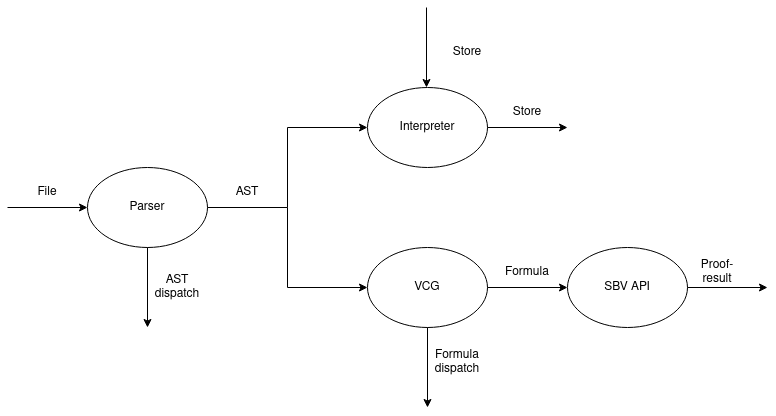
\includegraphics[width=\linewidth]{Implementation/IFCapp.png}
  \caption{Application layout for IFC}
  \label{fig:flow}
\end{figure}

\cref{sec:guide} explains how to interact with the application. In the \cref{sec:parser} to \cref{sec:api} we describe key points of the implementation, and \cref{sec:interface} describes an interface which allows for more general proofs about programs.

\subsection{Parser}\label{sec:parser}
The internal AST is defined pretty close to the grammar in \cref{table:grammar} and can be seen in Appendix \ref{}. Two matters are important to state about the parsing stage, ambiguity and ghost-variables.
\subsubsection{Grammar ambiguity}
For the parsing of a program we use the parser combinator library MegaParsec, which means we have to eliminate ambiguity in the grammar presented.
We do so in two different ways.
For arithmetic operators and boolean operators, we make use of the expression parser defined in \verb\Control.Monad.Combinators.Expr\.
This makes handling operators, precedence and associativity easy. Furthermore, it allows for easy extension with new operators.
For parsing the first order logic in assertions, we found the expression-parser unfit. One reason is that we want to allow for syntax ``forall x y z.'' to desugar to ``forall x. forall y. forall z''. Instead of using the expression-parser we manually introduce precedence, according to conventions, with negation most precedence, then conjuction and disjuction followed by quantifers and lastly implication. Furthermore the grammar has been left-factorized, as such.
\begin{figure}[h]
\begin{grammar}
<imp> ::= <quant> <imp'>

<imp'> ::= '$\Rightarrow$' <quant> <imp'> | $\epsilon$

<quant> ::= 'forall' <vname> '.' <quant>
\alt 'exists' <vname> '.' <quant>
\alt <cd>

<cd> ::= <neg> <cd'>

<cd'> ::= '$\wedge$' <neg> <cd'> | '$\vee$' <neg> <cd'> | $\epsilon$

<neg> ::= '$\sim$' <factor> | <factor>

<factor> ::=  <bexp> | '(' <imp> ')'
\end{grammar}

\end{figure}
We further introduces some syntactic sugar in the grammar such as ``if c \{s\};'' which will be desugared into ``if c \{s\} else \{skip\};''. However we dont need any special transformation other than using the  \verb\option\ parser-combinator.
\\~\\
For other parts of the grammar, which could have been syntactic sugar, such as implication and exist, we use the unsugared constructs. Although this introduces more code, the intent is to make the code easier to reason about in terms of the semantics. Furthermore it reads better in the output of the vc generator, and hence translate more directly into the predicate transformer semantics.
This at least has made the development process easier. Ideally this could be alleviated by a more comprehensible pretty-printer, but at the moment, we settle for a slightly bigger AST.

\subsubsection{Ghost variables}
As previously mentioned, it is semantically disallowed to use ghost-variables anywhere in the program-logic other than assertions. Although this is a semantical matter, we handle this in the parser. By simply fail to parse if a ghost variable appears anywhere not allowed, thus treating it as a syntactic issue.
We do so by adding a reader monadtransformer, to the internal transformer type \verb\parsecT\ of \verb\Megaparsec\.

\begin{lstlisting}{haskell}
type Parser = ParsecT Void String (ReaderT Bool Identity)
\end{lstlisting}

The boolean value in this environment will tell if the next parser (by the use of \verb\local\) must allow for parsing ghost variables. Which will certainly only happen in assertions.
% We find that eliminating illegal usecases for ghosts in the parser is far preferable than doing so in both the VC-generator and the evaluator, however this restricts us from generating ghost variables in our Quickcheck generation of statements.
% Having a local environment denoting if something is legal or not showed to be very useful, when handling assertions in the evaluator. An explanation of this can be seen in \cref{sec:evaluator}.


\subsection{Interpreter}\label{sec:evaluator}
The interpreter follows directly from the semantics presented in \cref{sec:Language}.
That is the intial store provided to the evalutor will be modified over the course of the program according to the semantics.
We define the \verb\Eval\ type as follows such:

\begin{lstlisting}
type STEnv = M.Map VName Integer
type Eval a = RWST () () STEnv (Either String) a
\end{lstlisting}

At the moment there is no use for neither \verb\reader\ nor \verb\writer\, however when the language in the future is extended to have procedures the reader monad will be a natural choice for the scoping rules of said procedures.
Likewise it is highly likely that the language would need to support some sort of output in the future.
The store described in \cref{sec:Language} is kept in the State \verb\STEnv\.
The store is simply a map from \texttt{VNames} to \texttt{Integers}. We want the store to be a State as the store after one monadic action should be chained with the next monadic action. This ensures that all variables are in scope for the rest of the program and hereby entails mutability.
Duly note that ghost variables will also reside in this environment but will not be mutable or even callable, as previously explained.
We make use of the error monad to resolve any runtime-errors that would arise, that is if a violation occurs, a ghost is assigned, a variable is used before it is defined, or if undefined behaviour arises such as division by 0. Semantically, the first error that occurs will be the return value of the computation.
\\~\\
Each type defined in the AST, \verb\Stmt\, \verb\FOL\, \verb\AExpr\, \verb\BExpr\ is evaluated by different functions which all operate under the \verb\Eval\ monad, which allows for a clean and modular monadic compiler. They have the following types:
%\footnote{Can we use a typeclass so they all are named eval??? Or is that too Rusty???}

\begin{lstlisting}
eval :: Stmt -> Eval ()
evalFOL :: FOL -> Eval Bool
evalBExpr :: BExpr -> Eval Bool
evalAExpr :: AExpr -> Eval Integer
\end{lstlisting}

From this we notice that all of the different constructs except for \verb\Stmt\, will produce a value, whereas \verb\Stmt\ can only produce monadic actions, in terms of modifying the store. This monadic context allows us to translate the operational semantics almost directly into Haskell code.
\cref{fig:evalS} presents the code for evaluating statements.

\begin{figure}[h]
\begin{lstlisting}
eval :: Stmt -> Eval ()
eval (Seq s1 s2) = eval s1 >> eval s2
eval (GhostAss vname a) =
    get >>= maybe (update vname a) (const _e) . M.lookup vname
eval (Assign vname a) = update vname a
eval (If c s1 s2) =
    evalBExpr c >>= \c' -> if c' then eval s1 else eval s2
eval (Asst f) = evalFOL f >>= \case
  True  -> return ()
  False -> _e
eval w@(While c invs _var s) =
  evalFOL invs >>= \case
    False -> _e
    True -> evalBExpr c >>= \case
      True -> eval s >> eval w
      False -> return ()
eval Skip = return ()
eval Fail = _e
\end{lstlisting}
\caption{Evaluator for statements.\footnote{Note that \verb\_e\ is a placeholder for the run-time errors mentioned before.}}
\label{fig:evalS}
\end{figure}

The most complex argument for equivalence between the code and the semantics is the \texttt{while} construct. \cref{fig:evalS}, line 11-16, shows how we evaluate it.
We first evaluate the invariant, to directly follow the semantical rules. Hence, when the invariant does not hold, we handle this case as abnormal termination, as per rule \textit{while-i-false} from \cref{table:semantic}, similarly to how we would do for a standard assertion.
If the invariant holds, but the loop-condition does not, we do nothing, as per rule \textit{while-false}.
Lastly if both the invariant and the loop-condition evaluates to \textit{true}, we evaluate the body, and then we evaluate the while loop again.
The other statements are simple and we treat them similarly to \texttt{while}, directly in accordance with the semantics.
\\~\\
One important note about the interpreter is that we have no good way of checking assertions which includes quantifiers. 
The reasons is that we wanted to support arbitrary precision integers.
This entails that we currently have no feasible way to check such assertions.
A potential solution would be to generate a symbolic reprensentation of the formula and try to satisfy it by using an external prover.
A downside to this approach is that the interpreter would then also require external dependencies, and not be a standalone program anymore.
All in all, this is unideal, and currently the approach is to ignore such assertions by considering them true. 
In \cref{sec:future} we describe a potential extension to \textit{While}, which could help alleviate this problem.
Non-quantified assertions are still evaluated as per the operational semantics.


\subsection{Verification Condition Generator}
The verification condition generator, uses the weakest precondition calculus to construct the condition, or weakest liberal precondition (if while has no specified variant). Again we want to be able to chain the actions and include a state and reader environment in the construction of the verification condition.

\begin{lstlisting}
type Counter = M.Map VName Count
type Env = M.Map VName VName
type WP a = StateT Counter (ReaderT Env (Either String)) a
\end{lstlisting}

The Counter state is used to give unique names to variables. Whereas we want the reader environment to resolve variable substitution in the formula generated from the weakest preconditions.
\\~\\
As described in \autoref{sec:vcg}, we use the quantified rule for assignment, when encountering assignments. In the development process we considered two different approaches to resolve this.

\subsubsection{First approach}
The initial approach tried to resolve $Q$ only after the entire formula were build. This would allows for WLP to be resolve in only two passes, one over the imperative language AST and one over Assertion Language AST in the formula. The approach was intended to build up a map as such, where \verb\VName\ is an identifier (String):

\begin{lstlisting}
type Env1 = M.Map VName [VName]
\end{lstlisting}

Whenever encountering a variable we would add a unique identifier to its value-list along with extending $Q$ by the WP rules, as such:

\begin{lstlisting}
missing
\end{lstlisting}

The result of running WP will then give a partially resolved formula and the final state. When resolving ... Jeg tænker lige.

\subsubsection{Second approach}
The second and current approach is to resolve $Q$ whenever we encounters an assignment. We generate the forall as such:
\begin{lstlisting}
wp (Assign x a) q = do
    x' <- genVar x
    q' <- local (M.insert x x') $ resolveQ1 q
    return $ Forall x' (Cond (RBinary Eq (Var x') a) .=>. q')
\end{lstlisting}
We make a new variable (by generating a unique identifier, based on the State), then we proceed to resolve $q$ with the new environment, such that every occurence of variable $x$ will be substituted by the newly generatd varaible $x'$. The \verb\Aexpr\ which $x$ evaluates to should not be resolved yet, as this will potentially depend on variables not yet encounted.
\\~\\
This approach is quite inefficient since it will go over the entire formula every time an assignment is made. Hence why we considered the other approach initially.
\\~\\
Because of their uniqueness ghost variables on the other hand is straight forward to resolve as we need no substitution.
\\~\\
Furthermore the current version does not enforce the formula to be closed, although it will be necessary in the generation of symbolic variables. Although easily fixed by a simple new iteration over the AST of the formula, and checking if any non-ghost variable does not contain a \verb\#\, we find that since the formula is intended to be fed to the next stage in the compiler it is uneccesary to do so.

\subsubsection{While - invariants and variants}
The \verb\while\ construct is the most complicated of the constructs. As previously mentioned, for partial correctness, we need atleast an invariant, and for full correctness also a variant. Hereby we enfore the user to provide as a minimum the invariant. The code for while is thus also quite complex compared to the rest:
\begin{lstlisting}
wp (While _b [] _var _s) _q = -- ERROR
wp (While b inv var s) q = do
  let invs = foldr1 (./\.) inv   -- Foldr all invariants
  st <- get
  -- Give back condition for unbounded integer variant
  (fa, var', veq) <- maybe (return
                            (id,
                            Cond $ BoolConst True,
                            Cond $ BoolConst True)) resolveVar var
  -- wp(s, I /\ invariant condition)
  w <- wp s (invs ./\. var')
  -- check which variables we wanna forall over
  fas <- findVars s []
  let inner = fa (((Cond b ./\. invs ./\. veq) .=>. w)
                          ./\. ((anegate (Cond b) ./\. invs) .=>. q))
  --- Fix the bound variables and resolve them
  env <- ask
  let env' = foldr (\\(x,y) a -> M.insert x y a) env fas
  inner' <- local (const env') $ resolveQ1 inner
  let fas' = foldr (Forall . snd) inner' fas
  return $ invs ./\. fas'
  where
    resolveVar :: Variant -> WP (FOL -> FOL, FOL, FOL)
    resolveVar var = do
      x <- genVar "variant"
      return (Forall x,
              Cond (Negate (RBinary Greater (IntConst 0) (Var x)))
               ./\. Cond (RBinary Less var (Var x))
             , Cond (RBinary Eq (Var x) var)
             )
\end{lstlisting}
If no invariant is provided an error is reported.
As mentioned in \autoref{sec:Language} we allow for syntactically providing multiple invariants, which should then all hold under conjuction.
We have tried to make the code generic in terms existence of the variant to eliminate code duplication.
line 6-9, will generate the conditions needed for the variant.
In case no variant is defined we use that predicate-logic and conjuction forms a monoid with $\top$ as identity element, such that, we generate no new $\forall$-quantification, and have subformular $b \Rightarrow WP(s,b)$.
Is there a variant, we generate the equality $\xi = v$, along with the well-founded relation for unbounded integers. This approach should translate pretty well, with possible other types that have a well-founded relation. The rest of the code simply checks which variables are assigned in the body of the while-loop, and generate a variable for each. Collectively this code will generate the weakest precondition for a while statement as per described in equation~\ref{eq:wpwhile}.


\subsection{proof-assistant API}
The proof-assistant API uses the SMT Based Verification library (SBV), which tries to simplify symbolic programming in Haskell. The library is quite generic and extensive compared to what we use it for.
We mostly make use of the higher level functions and dont mess with any of the internals, however the default type of SBV does not quite fit our needs.
Instead we use the provided transformer \texttt{SymbolicT}, such that we can embed the \texttt{Except} monad. We want to do so, as when iterating over the formular, we might encounter a variables not yet defined and here fail gracefully, instead of throwing an error.
The code which generates a \verb\Predicate ~ Sym SBool\ is simple, since the formula generated in the previous stage, will be already first order logic formula, which straight forwardly can be converted into SBV's types. For the entire highlevel logic we resolve it as simple as this:
\begin{lstlisting}
type Sym a = SymbolicT (ExceptT String IO) a
type SymTable = M.Map VName SInteger

fToS :: FOL -> SymTable -> Sym SBool
fToS (Cond b) st = bToS b st
fToS (Forall x a) st = forAll [x] $ \(x'::SInteger) ->
  fToS a (M.insert x x' st)
fToS (Exists x a) st = forSome [x] $ \(x'::SInteger) ->
  fToS a (M.insert x x' st)
fToS (ANegate a) st = sNot <$> fToS a st
fToS (AConj a b) st = onlM2 (.&&) (`fToS` st) a b
fToS (ADisj a b) st = onlM2 (.||) (`fToS` st) a b
fToS (AImp a b) st = onlM2 (.=>) (`fToS` st) a b
\end{lstlisting}

And equally easy it is to resolve \verb\bexpr\ and \verb\aexpr\. Ideally we would add a ReaderT to the transformer-stack to get rid of the explicit state.
We have not been able to resolve the type for this, because of the following type constraint \texttt{forAll :: MProvable m a => [String] -> a -> SymbolicT m SBool}, and \texttt{m} must be an \texttt{ExtractIO}, of which Reader and State cannot be implemented\cite{}.
The predicate constructed by traversing the formula from the last stage will then be used as argument for the SBV function \verb\prove\, which will try to prove the predicate using Z3.
If the program can correctly be proved by the external SMT solver, the output will be \texttt{Q.E.D.}
, whereas if the formula cannot be proved, a falsifiable instance of the variables will be presented.
For instance the output of the following program will obviously always be falsified.
\begin{lstlisting}
violate;
\end{lstlisting}
whereas the multiplication program in \cref{figure:mult} is proveable.


\subsection{Interface for proofs}\label{sec:interface}
As may have been apparant from the example programs presented earlier in this report, we requires each IFC program to have a header that looks as follows:
\begin{lstlisting}
vars: [ <variables> ]
requirements: { <preconditions> }
<!=_=!>
\end{lstlisting}
where <variables> describes the variables, which is initially in the ``store'' and <preconditions> is an assertion, which specifies a condition that should hold before the program starts.
The header does not provide anything new to the evaluator, (although we prepend the requirement to the program as an assertion), but it enables us to make more generic proofs about said programs.
In the current state, there is no procedures in IFC, which makes it difficult to reason about the input of variables, when trying to prove the weakest precondition, hence why we define said header.
The inspiration comes from how the whyML language defines procedures.
\autoref{fig:why3} is a whyML program equivalent to the mult.ifc program.
\begin{figure}[h]
\begin{lstlisting}
module Mult

  use int.Int
  use ref.Refint

  let mult (&q : ref int) (r: int) : int
    requires { q >= 0 && r >= 0 }
    =
    let ref res = 0 in
    let ghost a = q in
    while q > 0 do
      invariant { res = (a - q) * r && q >= 0}
      variant { q }
      decr q;
      res += r
    done;
    assert { res = a * r };
    res
end
\end{lstlisting}
\caption{Why3 program equivalent to mult.ifc}
\label{fig:why3}
\end{figure}
It is possible for why3 to generate a vector of input variables and then a precondition for each the \verb\requires\, such that $\forall x_{1},...,x_{n}. \; requires => WP(body, ensures)$.
That is whenever the requires holds, then the weakest precondition of the body should hold, where ensures states the postcondition. Notice that \autoref{fig:why3} does not use an ``ensures''. We define it this way as it more closely resemples our language.
And since we dont have any return values, we dont really need the ensures, since this might as well be part of the actual program.\footnote{is this clear if you dont know whyML?}

